\documentclass[a4paper]{book}
\usepackage{makeidx}
\usepackage{graphicx}
\usepackage{multicol}
\usepackage{float}
\usepackage{listings}
\usepackage{color}
\usepackage{ifthen}
\usepackage[table]{xcolor}
\usepackage{textcomp}
\usepackage{alltt}
\usepackage{ifpdf}
\ifpdf
\usepackage[pdftex,
            pagebackref=true,
            colorlinks=true,
            linkcolor=blue,
            unicode
           ]{hyperref}
\else
\usepackage[ps2pdf,
            pagebackref=true,
            colorlinks=true,
            linkcolor=blue,
            unicode
           ]{hyperref}
\usepackage{pspicture}
\fi
\usepackage[utf8]{inputenc}
\usepackage{mathptmx}
\usepackage[scaled=.90]{helvet}
\usepackage{courier}
\usepackage{doxygen}
\lstset{language=C++,inputencoding=utf8,basicstyle=\footnotesize,breaklines=true,breakatwhitespace=true,tabsize=8,numbers=left }
\makeindex
\setcounter{tocdepth}{3}
\renewcommand{\footrulewidth}{0.4pt}
\begin{document}
\hypersetup{pageanchor=false}
\begin{titlepage}
\vspace*{7cm}
\begin{center}
{\Large Baralho }\\
\vspace*{1cm}
{\large Generated by Doxygen 1.7.3}\\
\vspace*{0.5cm}
{\small Wed May 16 2012 22:41:07}\\
\end{center}
\end{titlepage}
\clearemptydoublepage
\pagenumbering{roman}
\tableofcontents
\clearemptydoublepage
\pagenumbering{arabic}
\hypersetup{pageanchor=true}
\chapter{Namespace Index}
\section{Packages}
Here are the packages with brief descriptions (if available):\begin{DoxyCompactList}
\item\contentsline{section}{\hyperlink{namespace_baralho}{Baralho} }{\pageref{namespace_baralho}}{}
\item\contentsline{section}{\hyperlink{namespace_exce_xC3_xA7_xC3_xB5es}{Exceções} }{\pageref{namespace_exce_xC3_xA7_xC3_xB5es}}{}
\end{DoxyCompactList}

\chapter{Class Index}
\section{\-Class \-Hierarchy}
\-This inheritance list is sorted roughly, but not completely, alphabetically\-:\begin{DoxyCompactList}
\item \contentsline{section}{\-Baralho.\-Baralho}{\pageref{class_baralho_1_1_baralho}}{}
\item \contentsline{section}{\-Baralho.\-Carta}{\pageref{class_baralho_1_1_carta}}{}
\item \contentsline{section}{\-Exceções.\-Carta\-Inexistente\-Exception}{\pageref{class_exce_xC3_xA7_xC3_xB5es_1_1_carta_inexistente_exception}}{}
\item \contentsline{section}{\-Exceções.\-Carta\-Invalida\-Exception}{\pageref{class_exce_xC3_xA7_xC3_xB5es_1_1_carta_invalida_exception}}{}
\item \contentsline{section}{\-Baralho.\-Compara\-Cartas}{\pageref{interface_baralho_1_1_compara_cartas}}{}
\begin{DoxyCompactList}
\item \contentsline{section}{\-Baralho.\-Comparacao\-Simples}{\pageref{class_baralho_1_1_comparacao_simples}}{}
\end{DoxyCompactList}
\item \contentsline{section}{\-Baralho.\-Monte}{\pageref{class_baralho_1_1_monte}}{}
\begin{DoxyCompactList}
\item \contentsline{section}{\-Baralho.\-Monte\-Comum}{\pageref{class_baralho_1_1_monte_comum}}{}
\item \contentsline{section}{\-Baralho.\-Monte\-Descarte}{\pageref{class_baralho_1_1_monte_descarte}}{}
\end{DoxyCompactList}
\item \contentsline{section}{\-Exceções.\-Sequencia\-Invalida\-Exception}{\pageref{class_exce_xC3_xA7_xC3_xB5es_1_1_sequencia_invalida_exception}}{}
\end{DoxyCompactList}

\chapter{Class Index}
\section{Estruturas de Dados}
Aqui estão as estruturas de dados, uniões e suas respectivas descrições\-:\begin{DoxyCompactList}
\item\contentsline{section}{\hyperlink{structbaralho}{baralho} }{\pageref{structbaralho}}{}
\end{DoxyCompactList}

\chapter{File Index}
\section{Lista de Arquivos}
Esta é a lista de todos os arquivos e suas respectivas descrições:\begin{DoxyCompactList}
\item\contentsline{section}{\hyperlink{corta_8c}{corta.c} }{\pageref{corta_8c}}{}
\item\contentsline{section}{\hyperlink{corta_8h}{corta.h} }{\pageref{corta_8h}}{}
\item\contentsline{section}{\hyperlink{embaralhar_8c}{embaralhar.c} }{\pageref{embaralhar_8c}}{}
\item\contentsline{section}{\hyperlink{embaralhar_8h}{embaralhar.h} }{\pageref{embaralhar_8h}}{}
\item\contentsline{section}{\hyperlink{retira_8c}{retira.c} }{\pageref{retira_8c}}{}
\item\contentsline{section}{\hyperlink{retira_8h}{retira.h} }{\pageref{retira_8h}}{}
\end{DoxyCompactList}

\chapter{Namespace Documentation}
\hypertarget{namespace_baralho}{
\section{\-Package \-Baralho}
\label{namespace_baralho}\index{\-Baralho@{\-Baralho}}
}
\subsection*{\-Classes}
\begin{DoxyCompactItemize}
\item 
class \hyperlink{class_baralho_1_1_baralho}{\-Baralho}
\item 
class \hyperlink{class_baralho_1_1_carta}{\-Carta}
\item 
class \hyperlink{class_baralho_1_1_comparacao_simples}{\-Comparacao\-Simples}
\item 
interface \hyperlink{interface_baralho_1_1_compara_cartas}{\-Compara\-Cartas}
\item 
class \hyperlink{class_baralho_1_1_monte}{\-Monte}
\item 
class \hyperlink{class_baralho_1_1_monte_comum}{\-Monte\-Comum}
\item 
class \hyperlink{class_baralho_1_1_monte_descarte}{\-Monte\-Descarte}
\end{DoxyCompactItemize}
\subsection*{\-Enumerations}
\begin{DoxyCompactItemize}
\item 
enum \hyperlink{namespace_baralho_ab887857dcb81ef6672322ce80039b905}{\-Naipe} \{ \hyperlink{namespace_baralho_ab887857dcb81ef6672322ce80039b905}{\-O\-U\-R\-O\-S}, 
\hyperlink{namespace_baralho_ab887857dcb81ef6672322ce80039b905}{peso}, 
\hyperlink{namespace_baralho_ab887857dcb81ef6672322ce80039b905}{peso}, 
\hyperlink{namespace_baralho_ab887857dcb81ef6672322ce80039b905}{peso}
 \}
\end{DoxyCompactItemize}


\subsection{\-Enumeration \-Type \-Documentation}
\hypertarget{namespace_baralho_ab887857dcb81ef6672322ce80039b905}{
\index{\-Baralho@{\-Baralho}!\-Naipe@{\-Naipe}}
\index{\-Naipe@{\-Naipe}!Baralho@{\-Baralho}}
\subsubsection[{\-Naipe}]{\setlength{\rightskip}{0pt plus 5cm}enum {\bf \-Baralho\-::\-Naipe}}}
\label{namespace_baralho_ab887857dcb81ef6672322ce80039b905}
\begin{Desc}
\item[\-Enumerator\-: ]\par
\begin{description}
\index{\-O\-U\-R\-O\-S@{\-O\-U\-R\-O\-S}!\-Baralho@{\-Baralho}}\index{\-Baralho@{\-Baralho}!\-O\-U\-R\-O\-S@{\-O\-U\-R\-O\-S}}\item[{\em 
\hypertarget{namespace_baralho_ab887857dcb81ef6672322ce80039b905}{
\-O\-U\-R\-O\-S}
\label{namespace_baralho_ab887857dcb81ef6672322ce80039b905}
}]\index{peso@{peso}!\-Baralho@{\-Baralho}}\index{\-Baralho@{\-Baralho}!peso@{peso}}\item[{\em 
\hypertarget{namespace_baralho_ab887857dcb81ef6672322ce80039b905}{
peso}
\label{namespace_baralho_ab887857dcb81ef6672322ce80039b905}
}]\index{peso@{peso}!\-Baralho@{\-Baralho}}\index{\-Baralho@{\-Baralho}!peso@{peso}}\item[{\em 
\hypertarget{namespace_baralho_ab887857dcb81ef6672322ce80039b905}{
peso}
\label{namespace_baralho_ab887857dcb81ef6672322ce80039b905}
}]\index{peso@{peso}!\-Baralho@{\-Baralho}}\index{\-Baralho@{\-Baralho}!peso@{peso}}\item[{\em 
\hypertarget{namespace_baralho_ab887857dcb81ef6672322ce80039b905}{
peso}
\label{namespace_baralho_ab887857dcb81ef6672322ce80039b905}
}]\end{description}
\end{Desc}


\hypertarget{namespace_exce_xC3_xA7_xC3_xB5es}{
\section{\-Package \-Exceções}
\label{namespace_exce_xC3_xA7_xC3_xB5es}\index{\-Exceções@{\-Exceções}}
}
\subsection*{\-Classes}
\begin{DoxyCompactItemize}
\item 
class \hyperlink{class_exce_xC3_xA7_xC3_xB5es_1_1_carta_inexistente_exception}{\-Carta\-Inexistente\-Exception}
\item 
class \hyperlink{class_exce_xC3_xA7_xC3_xB5es_1_1_carta_invalida_exception}{\-Carta\-Invalida\-Exception}
\item 
class \hyperlink{class_exce_xC3_xA7_xC3_xB5es_1_1_sequencia_invalida_exception}{\-Sequencia\-Invalida\-Exception}
\end{DoxyCompactItemize}

\chapter{Class Documentation}
\hypertarget{class_baralho_1_1_baralho}{
\section{\-Baralho.\-Baralho \-Class \-Reference}
\label{class_baralho_1_1_baralho}\index{\-Baralho.\-Baralho@{\-Baralho.\-Baralho}}
}
\subsection*{\-Public \-Member \-Functions}
\begin{DoxyCompactItemize}
\item 
\hyperlink{class_baralho_1_1_baralho_ab88f90bd08144f150e97b45bd63eadfd}{\-Baralho} (\hyperlink{class_baralho_1_1_monte}{\-Monte} monte\-Principal, \hyperlink{class_baralho_1_1_monte_descarte}{\-Monte\-Descarte} monte\-Descarte)
\item 
\hyperlink{class_baralho_1_1_baralho_a039c014d8bf91ceda3b003a1ee4d2418}{\-Baralho} (\hyperlink{class_baralho_1_1_monte}{\-Monte} monte\-Principal, \hyperlink{class_baralho_1_1_monte_descarte}{\-Monte\-Descarte} monte\-Descarte, \hyperlink{interface_baralho_1_1_compara_cartas}{\-Compara\-Cartas} forma\-Comparacao)
\item 
void \hyperlink{class_baralho_1_1_baralho_ae7ce198ebeadf6c0b3fb5ad109873f1c}{reiniciar\-Baralho} ()
\item 
void \hyperlink{class_baralho_1_1_baralho_a50716e1d93b3ed27800ac62b7b9e8b8a}{embaralhar} ()
\item 
void \hyperlink{class_baralho_1_1_baralho_a6839090e52620e5b665a12aceeba06f6}{cortar} (int ini, int fim)  throws Carta\-Inexistente\-Exception
\item 
\hyperlink{class_baralho_1_1_carta}{\-Carta} \hyperlink{class_baralho_1_1_baralho_a88c1b1eec22e717be39227ed2ceb9490}{retirar\-Carta\-Do\-Inicio} ()  throws Carta\-Inexistente\-Exception
\item 
\hyperlink{class_baralho_1_1_carta}{\-Carta} \hyperlink{class_baralho_1_1_baralho_a8441347c4eb47a0ba0f3bfbdfca59a9c}{retirar\-Carta\-Do\-Fim} ()  throws Carta\-Inexistente\-Exception 
\item 
void \hyperlink{class_baralho_1_1_baralho_a9df1c0a9c5c6c227b36e434248d5698d}{mover\-Do\-Inicio\-Para\-Fim} ()  throws Carta\-Inexistente\-Exception 
\item 
boolean \hyperlink{class_baralho_1_1_baralho_ad95b8caaaf2602be21923a9c02ab741f}{descartar} (\hyperlink{class_baralho_1_1_carta}{\-Carta} carta)
\item 
\hyperlink{class_baralho_1_1_carta}{\-Carta} \hyperlink{class_baralho_1_1_baralho_ad6ceed72b137e5bf5490af7dcd282648}{retirar\-Carta\-Do\-Descarte} (int pos)  throws Carta\-Inexistente\-Exception 
\item 
void \hyperlink{class_baralho_1_1_baralho_a9a20256555c03889f244ce40957ae7f8}{ver\-Carta\-Do\-Descarte} (int pos)  throws Carta\-Inexistente\-Exception 
\item 
int \hyperlink{class_baralho_1_1_baralho_ac382a9e91f65da63c8e3fac26eba6225}{tamanho} ()
\item 
int \hyperlink{class_baralho_1_1_baralho_aace43f8f3dbbca74e2e2b5083ec3f305}{tamanho\-Monte\-Principal} ()
\item 
int \hyperlink{class_baralho_1_1_baralho_a2c293b134d1b685b19e46376097c02b8}{tamanho\-Monte\-Descarte} ()
\end{DoxyCompactItemize}


\subsection{\-Detailed \-Description}
\-Classe que representa o baralho. \-O baralho conta com dois montes\-: \hyperlink{class_baralho_1_1_monte}{\-Monte} principal\-: monte inicial do baralho. \-O monte que sofre o corte e onde se compram as cartas. \hyperlink{class_baralho_1_1_monte}{\-Monte} de descarte\-: monte para vão as cartas descartadas pelos usuários do baralho. \begin{DoxyAuthor}{\-Author}
\-Rafael 
\end{DoxyAuthor}


\subsection{\-Constructor \& \-Destructor \-Documentation}
\hypertarget{class_baralho_1_1_baralho_ab88f90bd08144f150e97b45bd63eadfd}{
\index{\-Baralho\-::\-Baralho@{\-Baralho\-::\-Baralho}!\-Baralho@{\-Baralho}}
\index{\-Baralho@{\-Baralho}!Baralho::Baralho@{\-Baralho\-::\-Baralho}}
\subsubsection[{\-Baralho}]{\setlength{\rightskip}{0pt plus 5cm}\-Baralho.\-Baralho.\-Baralho (
\begin{DoxyParamCaption}
\item[{{\bf \-Monte}}]{monte\-Principal, }
\item[{{\bf \-Monte\-Descarte}}]{monte\-Descarte}
\end{DoxyParamCaption}
)}}
\label{class_baralho_1_1_baralho_ab88f90bd08144f150e97b45bd63eadfd}
\hypertarget{class_baralho_1_1_baralho_a039c014d8bf91ceda3b003a1ee4d2418}{
\index{\-Baralho\-::\-Baralho@{\-Baralho\-::\-Baralho}!\-Baralho@{\-Baralho}}
\index{\-Baralho@{\-Baralho}!Baralho::Baralho@{\-Baralho\-::\-Baralho}}
\subsubsection[{\-Baralho}]{\setlength{\rightskip}{0pt plus 5cm}\-Baralho.\-Baralho.\-Baralho (
\begin{DoxyParamCaption}
\item[{{\bf \-Monte}}]{monte\-Principal, }
\item[{{\bf \-Monte\-Descarte}}]{monte\-Descarte, }
\item[{{\bf \-Compara\-Cartas}}]{forma\-Comparacao}
\end{DoxyParamCaption}
)}}
\label{class_baralho_1_1_baralho_a039c014d8bf91ceda3b003a1ee4d2418}


\subsection{\-Member \-Function \-Documentation}
\hypertarget{class_baralho_1_1_baralho_a6839090e52620e5b665a12aceeba06f6}{
\index{\-Baralho\-::\-Baralho@{\-Baralho\-::\-Baralho}!cortar@{cortar}}
\index{cortar@{cortar}!Baralho::Baralho@{\-Baralho\-::\-Baralho}}
\subsubsection[{cortar}]{\setlength{\rightskip}{0pt plus 5cm}void \-Baralho.\-Baralho.\-cortar (
\begin{DoxyParamCaption}
\item[{int}]{ini, }
\item[{int}]{fim}
\end{DoxyParamCaption}
)  throws {\bf \-Carta\-Inexistente\-Exception}}}
\label{class_baralho_1_1_baralho_a6839090e52620e5b665a12aceeba06f6}
\-Faz um corte no baralho, ou seja, retira um conjunto de cartas do baralho e as passa para o topo. 
\begin{DoxyParams}{\-Parameters}
{\em ini} & -\/ \-Posição de onde começa o conjunto a ser retirado. \\
\hline
{\em fim} & -\/ \-Posição de onde termina o conjunto a ser retirado. \\
\hline
\end{DoxyParams}

\begin{DoxyExceptions}{\-Exceptions}
{\em \-Carta\-Inexistente\-Exception} & -\/ \-Caso alguma das posições (inicial ou final) especificada aponte para uma carta que não existe no monte. \\
\hline
\end{DoxyExceptions}
\hypertarget{class_baralho_1_1_baralho_ad95b8caaaf2602be21923a9c02ab741f}{
\index{\-Baralho\-::\-Baralho@{\-Baralho\-::\-Baralho}!descartar@{descartar}}
\index{descartar@{descartar}!Baralho::Baralho@{\-Baralho\-::\-Baralho}}
\subsubsection[{descartar}]{\setlength{\rightskip}{0pt plus 5cm}boolean \-Baralho.\-Baralho.\-descartar (
\begin{DoxyParamCaption}
\item[{{\bf \-Carta}}]{carta}
\end{DoxyParamCaption}
)}}
\label{class_baralho_1_1_baralho_ad95b8caaaf2602be21923a9c02ab741f}
\-Adiciona uma carta ao monte de descarte. 
\begin{DoxyParams}{\-Parameters}
{\em carta} & -\/ \hyperlink{class_baralho_1_1_carta}{\-Carta} a ser adicionada ao descarte. \\
\hline
\end{DoxyParams}
\begin{DoxyReturn}{\-Returns}
true se a carta foi adicionada ou false caso contrário. 
\end{DoxyReturn}
\hypertarget{class_baralho_1_1_baralho_a50716e1d93b3ed27800ac62b7b9e8b8a}{
\index{\-Baralho\-::\-Baralho@{\-Baralho\-::\-Baralho}!embaralhar@{embaralhar}}
\index{embaralhar@{embaralhar}!Baralho::Baralho@{\-Baralho\-::\-Baralho}}
\subsubsection[{embaralhar}]{\setlength{\rightskip}{0pt plus 5cm}void \-Baralho.\-Baralho.\-embaralhar (
\begin{DoxyParamCaption}
{}
\end{DoxyParamCaption}
)}}
\label{class_baralho_1_1_baralho_a50716e1d93b3ed27800ac62b7b9e8b8a}
\-Embaralha as cartas do baralho. \hypertarget{class_baralho_1_1_baralho_a9df1c0a9c5c6c227b36e434248d5698d}{
\index{\-Baralho\-::\-Baralho@{\-Baralho\-::\-Baralho}!mover\-Do\-Inicio\-Para\-Fim@{mover\-Do\-Inicio\-Para\-Fim}}
\index{mover\-Do\-Inicio\-Para\-Fim@{mover\-Do\-Inicio\-Para\-Fim}!Baralho::Baralho@{\-Baralho\-::\-Baralho}}
\subsubsection[{mover\-Do\-Inicio\-Para\-Fim}]{\setlength{\rightskip}{0pt plus 5cm}void \-Baralho.\-Baralho.\-mover\-Do\-Inicio\-Para\-Fim (
\begin{DoxyParamCaption}
{}
\end{DoxyParamCaption}
)  throws {\bf \-Carta\-Inexistente\-Exception} }}
\label{class_baralho_1_1_baralho_a9df1c0a9c5c6c227b36e434248d5698d}
\-Retira uma carta do topo do baralho e a passa para o início do baralho. 
\begin{DoxyExceptions}{\-Exceptions}
{\em \-Carta\-Inexistente\-Exception} & -\/ \-Caso não haja mais cartas no monte principal. \\
\hline
\end{DoxyExceptions}
\hypertarget{class_baralho_1_1_baralho_ae7ce198ebeadf6c0b3fb5ad109873f1c}{
\index{\-Baralho\-::\-Baralho@{\-Baralho\-::\-Baralho}!reiniciar\-Baralho@{reiniciar\-Baralho}}
\index{reiniciar\-Baralho@{reiniciar\-Baralho}!Baralho::Baralho@{\-Baralho\-::\-Baralho}}
\subsubsection[{reiniciar\-Baralho}]{\setlength{\rightskip}{0pt plus 5cm}void \-Baralho.\-Baralho.\-reiniciar\-Baralho (
\begin{DoxyParamCaption}
{}
\end{DoxyParamCaption}
)}}
\label{class_baralho_1_1_baralho_ae7ce198ebeadf6c0b3fb5ad109873f1c}
\-Elimina as cartas do monte e inicializa o baralho novamente (initialize()). \hypertarget{class_baralho_1_1_baralho_ad6ceed72b137e5bf5490af7dcd282648}{
\index{\-Baralho\-::\-Baralho@{\-Baralho\-::\-Baralho}!retirar\-Carta\-Do\-Descarte@{retirar\-Carta\-Do\-Descarte}}
\index{retirar\-Carta\-Do\-Descarte@{retirar\-Carta\-Do\-Descarte}!Baralho::Baralho@{\-Baralho\-::\-Baralho}}
\subsubsection[{retirar\-Carta\-Do\-Descarte}]{\setlength{\rightskip}{0pt plus 5cm}{\bf \-Carta} \-Baralho.\-Baralho.\-retirar\-Carta\-Do\-Descarte (
\begin{DoxyParamCaption}
\item[{int}]{pos}
\end{DoxyParamCaption}
)  throws {\bf \-Carta\-Inexistente\-Exception} }}
\label{class_baralho_1_1_baralho_ad6ceed72b137e5bf5490af7dcd282648}
\-Retira uma carta do monte de descarte. 
\begin{DoxyParams}{\-Parameters}
{\em pos} & -\/ \-Posição do monte de descarte de onde a carta será retirada. \\
\hline
\end{DoxyParams}
\begin{DoxyReturn}{\-Returns}
\-A carta, caso a posição especificada aponte para uma carta do monte. 
\end{DoxyReturn}

\begin{DoxyExceptions}{\-Exceptions}
{\em \-Carta\-Inexistente\-Exception} & -\/ \-Caso a posição especificada não aponte para uma carta no monte. \\
\hline
\end{DoxyExceptions}
\hypertarget{class_baralho_1_1_baralho_a8441347c4eb47a0ba0f3bfbdfca59a9c}{
\index{\-Baralho\-::\-Baralho@{\-Baralho\-::\-Baralho}!retirar\-Carta\-Do\-Fim@{retirar\-Carta\-Do\-Fim}}
\index{retirar\-Carta\-Do\-Fim@{retirar\-Carta\-Do\-Fim}!Baralho::Baralho@{\-Baralho\-::\-Baralho}}
\subsubsection[{retirar\-Carta\-Do\-Fim}]{\setlength{\rightskip}{0pt plus 5cm}{\bf \-Carta} \-Baralho.\-Baralho.\-retirar\-Carta\-Do\-Fim (
\begin{DoxyParamCaption}
{}
\end{DoxyParamCaption}
)  throws {\bf \-Carta\-Inexistente\-Exception} }}
\label{class_baralho_1_1_baralho_a8441347c4eb47a0ba0f3bfbdfca59a9c}
\-Retira uma carta do topo do monte principal. \begin{DoxyReturn}{\-Returns}
\hyperlink{class_baralho_1_1_carta}{\-Carta} -\/ \hyperlink{class_baralho_1_1_carta}{\-Carta} retidada do topo do monte principal 
\end{DoxyReturn}

\begin{DoxyExceptions}{\-Exceptions}
{\em \-Carta\-Inexistente\-Exception} & -\/ \-Caso não haja mais cartas no monte principal. \\
\hline
\end{DoxyExceptions}
\hypertarget{class_baralho_1_1_baralho_a88c1b1eec22e717be39227ed2ceb9490}{
\index{\-Baralho\-::\-Baralho@{\-Baralho\-::\-Baralho}!retirar\-Carta\-Do\-Inicio@{retirar\-Carta\-Do\-Inicio}}
\index{retirar\-Carta\-Do\-Inicio@{retirar\-Carta\-Do\-Inicio}!Baralho::Baralho@{\-Baralho\-::\-Baralho}}
\subsubsection[{retirar\-Carta\-Do\-Inicio}]{\setlength{\rightskip}{0pt plus 5cm}{\bf \-Carta} \-Baralho.\-Baralho.\-retirar\-Carta\-Do\-Inicio (
\begin{DoxyParamCaption}
{}
\end{DoxyParamCaption}
)  throws {\bf \-Carta\-Inexistente\-Exception}}}
\label{class_baralho_1_1_baralho_a88c1b1eec22e717be39227ed2ceb9490}
\-Retira uma carta do início do monte principal. \begin{DoxyReturn}{\-Returns}
\hyperlink{class_baralho_1_1_carta}{\-Carta} -\/ \hyperlink{class_baralho_1_1_carta}{\-Carta} retirada do início do baralho. 
\end{DoxyReturn}

\begin{DoxyExceptions}{\-Exceptions}
{\em \-Carta\-Inexistente\-Exception} & -\/ \-Caso não haja mais cartas no monte principal. \\
\hline
\end{DoxyExceptions}
\hypertarget{class_baralho_1_1_baralho_ac382a9e91f65da63c8e3fac26eba6225}{
\index{\-Baralho\-::\-Baralho@{\-Baralho\-::\-Baralho}!tamanho@{tamanho}}
\index{tamanho@{tamanho}!Baralho::Baralho@{\-Baralho\-::\-Baralho}}
\subsubsection[{tamanho}]{\setlength{\rightskip}{0pt plus 5cm}int \-Baralho.\-Baralho.\-tamanho (
\begin{DoxyParamCaption}
{}
\end{DoxyParamCaption}
)}}
\label{class_baralho_1_1_baralho_ac382a9e91f65da63c8e3fac26eba6225}
\-Retorna o tamanho do baralho. \-O tamanho do baralho é dado pela soma do tamanho do monte principal com o tamanho do monte de descarte. \begin{DoxyReturn}{\-Returns}
\-Tamanho do baralho. 
\end{DoxyReturn}
\hypertarget{class_baralho_1_1_baralho_a2c293b134d1b685b19e46376097c02b8}{
\index{\-Baralho\-::\-Baralho@{\-Baralho\-::\-Baralho}!tamanho\-Monte\-Descarte@{tamanho\-Monte\-Descarte}}
\index{tamanho\-Monte\-Descarte@{tamanho\-Monte\-Descarte}!Baralho::Baralho@{\-Baralho\-::\-Baralho}}
\subsubsection[{tamanho\-Monte\-Descarte}]{\setlength{\rightskip}{0pt plus 5cm}int \-Baralho.\-Baralho.\-tamanho\-Monte\-Descarte (
\begin{DoxyParamCaption}
{}
\end{DoxyParamCaption}
)}}
\label{class_baralho_1_1_baralho_a2c293b134d1b685b19e46376097c02b8}
\-Retorna o tamanho do mont de descarte (quantidade de cartas). \begin{DoxyReturn}{\-Returns}
\-Tamanho do monte de descarte. 
\end{DoxyReturn}
\hypertarget{class_baralho_1_1_baralho_aace43f8f3dbbca74e2e2b5083ec3f305}{
\index{\-Baralho\-::\-Baralho@{\-Baralho\-::\-Baralho}!tamanho\-Monte\-Principal@{tamanho\-Monte\-Principal}}
\index{tamanho\-Monte\-Principal@{tamanho\-Monte\-Principal}!Baralho::Baralho@{\-Baralho\-::\-Baralho}}
\subsubsection[{tamanho\-Monte\-Principal}]{\setlength{\rightskip}{0pt plus 5cm}int \-Baralho.\-Baralho.\-tamanho\-Monte\-Principal (
\begin{DoxyParamCaption}
{}
\end{DoxyParamCaption}
)}}
\label{class_baralho_1_1_baralho_aace43f8f3dbbca74e2e2b5083ec3f305}
\-Retorna o tamanho do monte principal (quantidade de cartas). \begin{DoxyReturn}{\-Returns}
\-Tamanho do monte principal. 
\end{DoxyReturn}
\hypertarget{class_baralho_1_1_baralho_a9a20256555c03889f244ce40957ae7f8}{
\index{\-Baralho\-::\-Baralho@{\-Baralho\-::\-Baralho}!ver\-Carta\-Do\-Descarte@{ver\-Carta\-Do\-Descarte}}
\index{ver\-Carta\-Do\-Descarte@{ver\-Carta\-Do\-Descarte}!Baralho::Baralho@{\-Baralho\-::\-Baralho}}
\subsubsection[{ver\-Carta\-Do\-Descarte}]{\setlength{\rightskip}{0pt plus 5cm}void \-Baralho.\-Baralho.\-ver\-Carta\-Do\-Descarte (
\begin{DoxyParamCaption}
\item[{int}]{pos}
\end{DoxyParamCaption}
)  throws {\bf \-Carta\-Inexistente\-Exception} }}
\label{class_baralho_1_1_baralho_a9a20256555c03889f244ce40957ae7f8}
\-Exibe uma carta do monte de descarte. 
\begin{DoxyParams}{\-Parameters}
{\em pos} & -\/ \-Posição do monte de descarte que aponta para a carta a ser exibida. \\
\hline
\end{DoxyParams}

\begin{DoxyExceptions}{\-Exceptions}
{\em \-Carta\-Inexistente\-Exception} & -\/ \-Caso a posição especificada não aponte para uma carta no monte. \\
\hline
\end{DoxyExceptions}


\-The documentation for this class was generated from the following file\-:\begin{DoxyCompactItemize}
\item 
aula/111450026/\-Baralho/\-Baralho/\hyperlink{_baralho_8java}{\-Baralho.\-java}\end{DoxyCompactItemize}

\hypertarget{class_baralho_1_1_carta}{
\section{Baralho.Carta Class Reference}
\label{class_baralho_1_1_carta}\index{Baralho::Carta@{Baralho::Carta}}
}
\subsection*{Public Member Functions}
\begin{DoxyCompactItemize}
\item 
\hyperlink{class_baralho_1_1_carta_a0112885d7f19cccbe902005855eaf417}{Carta} (int valor, \hyperlink{namespace_baralho_ab887857dcb81ef6672322ce80039b905}{Naipe} naipe)  throws CartaInvalidaException
\item 
\hyperlink{class_baralho_1_1_carta_ab6f4c7de7f418095d9bad9587c457bea}{Carta} (int valor, \hyperlink{namespace_baralho_ab887857dcb81ef6672322ce80039b905}{Naipe} naipe, \hyperlink{interface_baralho_1_1_compara_cartas}{ComparaCartas} cp)  throws CartaInvalidaException
\item 
int \hyperlink{class_baralho_1_1_carta_a8cd63f6e252c1193bf10ec877f6982f8}{getValor} ()
\item 
\hyperlink{namespace_baralho_ab887857dcb81ef6672322ce80039b905}{Naipe} \hyperlink{class_baralho_1_1_carta_a327a805c7a73b5dce6538fd3f4c7f4ae}{getNaipe} ()
\item 
void \hyperlink{class_baralho_1_1_carta_a05361c159805fb0ad54f7b6a3d358019}{setComparaCartas} (\hyperlink{interface_baralho_1_1_compara_cartas}{ComparaCartas} cp)
\item 
int \hyperlink{class_baralho_1_1_carta_a7bc607ded2e593d2230c4cb0fb35b9d3}{getPesoCarta} ()
\item 
int \hyperlink{class_baralho_1_1_carta_a922703c5ca6a4c0aa2e7b50e5e0522b4}{hashCode} ()
\item 
boolean \hyperlink{class_baralho_1_1_carta_a834eb141943c980aa1c2d78c3c3a8541}{equals} (Object o)
\item 
String \hyperlink{class_baralho_1_1_carta_afd20dd3fad21790f281563e600ba7fe0}{toString} ()
\item 
boolean \hyperlink{class_baralho_1_1_carta_ab96ae30df37af13cb0ab42dcebd02f3e}{comparaCarta} (\hyperlink{class_baralho_1_1_carta}{Carta} carta)
\end{DoxyCompactItemize}


\subsection{Detailed Description}
Classe representativa de uma carta de baralho. Possui um valor (1,2,...,13) e um naipe (ouros, espadas, copas ou paus). \begin{DoxyAuthor}{Author}
Rafael 
\end{DoxyAuthor}


\subsection{Constructor \& Destructor Documentation}
\hypertarget{class_baralho_1_1_carta_a0112885d7f19cccbe902005855eaf417}{
\index{Baralho::Carta@{Baralho::Carta}!Carta@{Carta}}
\index{Carta@{Carta}!Baralho::Carta@{Baralho::Carta}}
\subsubsection[{Carta}]{\setlength{\rightskip}{0pt plus 5cm}Baralho.Carta.Carta (
\begin{DoxyParamCaption}
\item[{int}]{valor, }
\item[{{\bf Naipe}}]{naipe}
\end{DoxyParamCaption}
)  throws {\bf CartaInvalidaException}}}
\label{class_baralho_1_1_carta_a0112885d7f19cccbe902005855eaf417}
Construtor da classe carta. Lança uma exceção caso o valor da carta seja inválido. Por exemplo, valor 14 ou 0. 
\begin{DoxyParams}{Parameters}
{\em valor} & -\/ Valor da carta (1 à 13). \\
\hline
{\em naipe} & -\/ Naipe da carta (ouros, espadas, copas e paus). \\
\hline
\end{DoxyParams}

\begin{DoxyExceptions}{Exceptions}
{\em CartaInvalidaException} & -\/ Exceção lançada caso o valor da carta seja inválido. \\
\hline
\end{DoxyExceptions}
\hypertarget{class_baralho_1_1_carta_ab6f4c7de7f418095d9bad9587c457bea}{
\index{Baralho::Carta@{Baralho::Carta}!Carta@{Carta}}
\index{Carta@{Carta}!Baralho::Carta@{Baralho::Carta}}
\subsubsection[{Carta}]{\setlength{\rightskip}{0pt plus 5cm}Baralho.Carta.Carta (
\begin{DoxyParamCaption}
\item[{int}]{valor, }
\item[{{\bf Naipe}}]{naipe, }
\item[{{\bf ComparaCartas}}]{cp}
\end{DoxyParamCaption}
)  throws {\bf CartaInvalidaException}}}
\label{class_baralho_1_1_carta_ab6f4c7de7f418095d9bad9587c457bea}
Construtor da classe carta. Lança uma exceção caso o valor da carta seja inválido. Por exemplo, valor 14 ou 0. 
\begin{DoxyParams}{Parameters}
{\em valor} & -\/ Valor da carta (1 à 13). \\
\hline
{\em naipe} & -\/ Naipe da carta (ouros, espadas, copas e paus). \\
\hline
{\em cp} & -\/ Forma de comparação das cartas. \\
\hline
\end{DoxyParams}

\begin{DoxyExceptions}{Exceptions}
{\em CartaInvalidaException} & -\/ Exceção lançada caso o valor da carta seja inválido. \\
\hline
\end{DoxyExceptions}


\subsection{Member Function Documentation}
\hypertarget{class_baralho_1_1_carta_ab96ae30df37af13cb0ab42dcebd02f3e}{
\index{Baralho::Carta@{Baralho::Carta}!comparaCarta@{comparaCarta}}
\index{comparaCarta@{comparaCarta}!Baralho::Carta@{Baralho::Carta}}
\subsubsection[{comparaCarta}]{\setlength{\rightskip}{0pt plus 5cm}boolean Baralho.Carta.comparaCarta (
\begin{DoxyParamCaption}
\item[{{\bf Carta}}]{carta}
\end{DoxyParamCaption}
)}}
\label{class_baralho_1_1_carta_ab96ae30df37af13cb0ab42dcebd02f3e}
Compara com outra carta. 
\begin{DoxyParams}{Parameters}
{\em carta} & -\/ \hyperlink{class_baralho_1_1_carta}{Carta} a ser comparada. \\
\hline
\end{DoxyParams}
\begin{DoxyReturn}{Returns}
true -\/ Caso a carta com a qual está sendo comparada tiver peso menor ou igual. false -\/ Caso a carta com a qual está sendo comparada tiver peso maior. 
\end{DoxyReturn}
\hypertarget{class_baralho_1_1_carta_a834eb141943c980aa1c2d78c3c3a8541}{
\index{Baralho::Carta@{Baralho::Carta}!equals@{equals}}
\index{equals@{equals}!Baralho::Carta@{Baralho::Carta}}
\subsubsection[{equals}]{\setlength{\rightskip}{0pt plus 5cm}boolean Baralho.Carta.equals (
\begin{DoxyParamCaption}
\item[{Object}]{o}
\end{DoxyParamCaption}
)}}
\label{class_baralho_1_1_carta_a834eb141943c980aa1c2d78c3c3a8541}
Equals de Object sobreposto. Duas cartas são iguais se possuírem o mesmo valor e naipe. 
\begin{DoxyParams}{Parameters}
{\em o} & -\/ Object. \\
\hline
\end{DoxyParams}
\begin{DoxyReturn}{Returns}
-\/ true se iguais ou false caso contrário. 
\end{DoxyReturn}
\hypertarget{class_baralho_1_1_carta_a327a805c7a73b5dce6538fd3f4c7f4ae}{
\index{Baralho::Carta@{Baralho::Carta}!getNaipe@{getNaipe}}
\index{getNaipe@{getNaipe}!Baralho::Carta@{Baralho::Carta}}
\subsubsection[{getNaipe}]{\setlength{\rightskip}{0pt plus 5cm}{\bf Naipe} Baralho.Carta.getNaipe (
\begin{DoxyParamCaption}
{}
\end{DoxyParamCaption}
)}}
\label{class_baralho_1_1_carta_a327a805c7a73b5dce6538fd3f4c7f4ae}
Retorna o naipe da carta. \begin{DoxyReturn}{Returns}
naipe -\/ naipe da carta. 
\end{DoxyReturn}
\hypertarget{class_baralho_1_1_carta_a7bc607ded2e593d2230c4cb0fb35b9d3}{
\index{Baralho::Carta@{Baralho::Carta}!getPesoCarta@{getPesoCarta}}
\index{getPesoCarta@{getPesoCarta}!Baralho::Carta@{Baralho::Carta}}
\subsubsection[{getPesoCarta}]{\setlength{\rightskip}{0pt plus 5cm}int Baralho.Carta.getPesoCarta (
\begin{DoxyParamCaption}
{}
\end{DoxyParamCaption}
)}}
\label{class_baralho_1_1_carta_a7bc607ded2e593d2230c4cb0fb35b9d3}
Retorna o peso da carta. \begin{DoxyReturn}{Returns}
peso da carta. 
\end{DoxyReturn}
\hypertarget{class_baralho_1_1_carta_a8cd63f6e252c1193bf10ec877f6982f8}{
\index{Baralho::Carta@{Baralho::Carta}!getValor@{getValor}}
\index{getValor@{getValor}!Baralho::Carta@{Baralho::Carta}}
\subsubsection[{getValor}]{\setlength{\rightskip}{0pt plus 5cm}int Baralho.Carta.getValor (
\begin{DoxyParamCaption}
{}
\end{DoxyParamCaption}
)}}
\label{class_baralho_1_1_carta_a8cd63f6e252c1193bf10ec877f6982f8}
Retorna o valor da carta. \begin{DoxyReturn}{Returns}
valor -\/ valor da carta. 
\end{DoxyReturn}
\hypertarget{class_baralho_1_1_carta_a922703c5ca6a4c0aa2e7b50e5e0522b4}{
\index{Baralho::Carta@{Baralho::Carta}!hashCode@{hashCode}}
\index{hashCode@{hashCode}!Baralho::Carta@{Baralho::Carta}}
\subsubsection[{hashCode}]{\setlength{\rightskip}{0pt plus 5cm}int Baralho.Carta.hashCode (
\begin{DoxyParamCaption}
{}
\end{DoxyParamCaption}
)}}
\label{class_baralho_1_1_carta_a922703c5ca6a4c0aa2e7b50e5e0522b4}
HashCode do objeto (carta). Baseado no peso da carta. \begin{DoxyReturn}{Returns}
hashCode. 
\end{DoxyReturn}
\hypertarget{class_baralho_1_1_carta_a05361c159805fb0ad54f7b6a3d358019}{
\index{Baralho::Carta@{Baralho::Carta}!setComparaCartas@{setComparaCartas}}
\index{setComparaCartas@{setComparaCartas}!Baralho::Carta@{Baralho::Carta}}
\subsubsection[{setComparaCartas}]{\setlength{\rightskip}{0pt plus 5cm}void Baralho.Carta.setComparaCartas (
\begin{DoxyParamCaption}
\item[{{\bf ComparaCartas}}]{cp}
\end{DoxyParamCaption}
)}}
\label{class_baralho_1_1_carta_a05361c159805fb0ad54f7b6a3d358019}
Atribui a forma de comparar uma carta com outra. Pode variar de acordo com o jogo que as cartas estão sendo usadas. 
\begin{DoxyParams}{Parameters}
{\em cp} & -\/ Objeto responsável por comparar as cartas. \\
\hline
\end{DoxyParams}
\hypertarget{class_baralho_1_1_carta_afd20dd3fad21790f281563e600ba7fe0}{
\index{Baralho::Carta@{Baralho::Carta}!toString@{toString}}
\index{toString@{toString}!Baralho::Carta@{Baralho::Carta}}
\subsubsection[{toString}]{\setlength{\rightskip}{0pt plus 5cm}String Baralho.Carta.toString (
\begin{DoxyParamCaption}
{}
\end{DoxyParamCaption}
)}}
\label{class_baralho_1_1_carta_afd20dd3fad21790f281563e600ba7fe0}
toString de Object sobreposto. \char`\"{}Carta -\/ \char`\"{} + valor + \char`\"{} \char`\"{} + naipe". O valor pode ser a letra correspondente a carta. \begin{DoxyReturn}{Returns}
String -\/ Breve descrição da carta. 
\end{DoxyReturn}


The documentation for this class was generated from the following file:\begin{DoxyCompactItemize}
\item 
aula/111450026/Trabalho Baralho/Baralho/src/Baralho/\hyperlink{_carta_8java}{Carta.java}\end{DoxyCompactItemize}

\hypertarget{class_exce_xC3_xA7_xC3_xB5es_1_1_carta_inexistente_exception}{
\section{\-Exceções.\-Carta\-Inexistente\-Exception \-Class \-Reference}
\label{class_exce_xC3_xA7_xC3_xB5es_1_1_carta_inexistente_exception}\index{\-Exceções.\-Carta\-Inexistente\-Exception@{\-Exceções.\-Carta\-Inexistente\-Exception}}
}
\subsection*{\-Public \-Member \-Functions}
\begin{DoxyCompactItemize}
\item 
\hyperlink{class_exce_xC3_xA7_xC3_xB5es_1_1_carta_inexistente_exception_ab4926babd32689f2b9891911619e8938}{\-Carta\-Inexistente\-Exception} (\-String s)
\item 
\-String \hyperlink{class_exce_xC3_xA7_xC3_xB5es_1_1_carta_inexistente_exception_ac14b587ceb45140077d423dbc8a21faa}{get\-Message} ()
\end{DoxyCompactItemize}


\subsection{\-Detailed \-Description}
\begin{DoxyAuthor}{\-Author}
pc 
\end{DoxyAuthor}


\subsection{\-Constructor \& \-Destructor \-Documentation}
\hypertarget{class_exce_xC3_xA7_xC3_xB5es_1_1_carta_inexistente_exception_ab4926babd32689f2b9891911619e8938}{
\index{\-Exceções\-::\-Carta\-Inexistente\-Exception@{\-Exceções\-::\-Carta\-Inexistente\-Exception}!\-Carta\-Inexistente\-Exception@{\-Carta\-Inexistente\-Exception}}
\index{\-Carta\-Inexistente\-Exception@{\-Carta\-Inexistente\-Exception}!Exceções::CartaInexistenteException@{\-Exceções\-::\-Carta\-Inexistente\-Exception}}
\subsubsection[{\-Carta\-Inexistente\-Exception}]{\setlength{\rightskip}{0pt plus 5cm}\-Exceções.\-Carta\-Inexistente\-Exception.\-Carta\-Inexistente\-Exception (
\begin{DoxyParamCaption}
\item[{\-String}]{s}
\end{DoxyParamCaption}
)}}
\label{class_exce_xC3_xA7_xC3_xB5es_1_1_carta_inexistente_exception_ab4926babd32689f2b9891911619e8938}


\subsection{\-Member \-Function \-Documentation}
\hypertarget{class_exce_xC3_xA7_xC3_xB5es_1_1_carta_inexistente_exception_ac14b587ceb45140077d423dbc8a21faa}{
\index{\-Exceções\-::\-Carta\-Inexistente\-Exception@{\-Exceções\-::\-Carta\-Inexistente\-Exception}!get\-Message@{get\-Message}}
\index{get\-Message@{get\-Message}!Exceções::CartaInexistenteException@{\-Exceções\-::\-Carta\-Inexistente\-Exception}}
\subsubsection[{get\-Message}]{\setlength{\rightskip}{0pt plus 5cm}\-String \-Exceções.\-Carta\-Inexistente\-Exception.\-get\-Message (
\begin{DoxyParamCaption}
{}
\end{DoxyParamCaption}
)}}
\label{class_exce_xC3_xA7_xC3_xB5es_1_1_carta_inexistente_exception_ac14b587ceb45140077d423dbc8a21faa}


\-The documentation for this class was generated from the following file\-:\begin{DoxyCompactItemize}
\item 
aula/111450026/\-Trabalho Baralho/\-Baralho/src/\-Exceções/\hyperlink{_carta_inexistente_exception_8java}{\-Carta\-Inexistente\-Exception.\-java}\end{DoxyCompactItemize}

\hypertarget{class_exce_xC3_xA7_xC3_xB5es_1_1_carta_invalida_exception}{
\section{\-Exceções.\-Carta\-Invalida\-Exception \-Class \-Reference}
\label{class_exce_xC3_xA7_xC3_xB5es_1_1_carta_invalida_exception}\index{\-Exceções.\-Carta\-Invalida\-Exception@{\-Exceções.\-Carta\-Invalida\-Exception}}
}
\subsection*{\-Public \-Member \-Functions}
\begin{DoxyCompactItemize}
\item 
\hyperlink{class_exce_xC3_xA7_xC3_xB5es_1_1_carta_invalida_exception_aae435dd72af4ee38c188dcb041bae265}{\-Carta\-Invalida\-Exception} (\-String s, int valor\-Carta, \-String naipe\-Carta)
\item 
\-String \hyperlink{class_exce_xC3_xA7_xC3_xB5es_1_1_carta_invalida_exception_a12270c88daf2f27858e9e6e654c7903a}{get\-Message} ()
\end{DoxyCompactItemize}


\subsection{\-Detailed \-Description}
\begin{DoxyAuthor}{\-Author}
pc 
\end{DoxyAuthor}


\subsection{\-Constructor \& \-Destructor \-Documentation}
\hypertarget{class_exce_xC3_xA7_xC3_xB5es_1_1_carta_invalida_exception_aae435dd72af4ee38c188dcb041bae265}{
\index{\-Exceções\-::\-Carta\-Invalida\-Exception@{\-Exceções\-::\-Carta\-Invalida\-Exception}!\-Carta\-Invalida\-Exception@{\-Carta\-Invalida\-Exception}}
\index{\-Carta\-Invalida\-Exception@{\-Carta\-Invalida\-Exception}!Exceções::CartaInvalidaException@{\-Exceções\-::\-Carta\-Invalida\-Exception}}
\subsubsection[{\-Carta\-Invalida\-Exception}]{\setlength{\rightskip}{0pt plus 5cm}\-Exceções.\-Carta\-Invalida\-Exception.\-Carta\-Invalida\-Exception (
\begin{DoxyParamCaption}
\item[{\-String}]{s, }
\item[{int}]{valor\-Carta, }
\item[{\-String}]{naipe\-Carta}
\end{DoxyParamCaption}
)}}
\label{class_exce_xC3_xA7_xC3_xB5es_1_1_carta_invalida_exception_aae435dd72af4ee38c188dcb041bae265}


\subsection{\-Member \-Function \-Documentation}
\hypertarget{class_exce_xC3_xA7_xC3_xB5es_1_1_carta_invalida_exception_a12270c88daf2f27858e9e6e654c7903a}{
\index{\-Exceções\-::\-Carta\-Invalida\-Exception@{\-Exceções\-::\-Carta\-Invalida\-Exception}!get\-Message@{get\-Message}}
\index{get\-Message@{get\-Message}!Exceções::CartaInvalidaException@{\-Exceções\-::\-Carta\-Invalida\-Exception}}
\subsubsection[{get\-Message}]{\setlength{\rightskip}{0pt plus 5cm}\-String \-Exceções.\-Carta\-Invalida\-Exception.\-get\-Message (
\begin{DoxyParamCaption}
{}
\end{DoxyParamCaption}
)}}
\label{class_exce_xC3_xA7_xC3_xB5es_1_1_carta_invalida_exception_a12270c88daf2f27858e9e6e654c7903a}


\-The documentation for this class was generated from the following file\-:\begin{DoxyCompactItemize}
\item 
aula/111450026/\-Trabalho Baralho/\-Baralho/src/\-Exceções/\hyperlink{_carta_invalida_exception_8java}{\-Carta\-Invalida\-Exception.\-java}\end{DoxyCompactItemize}

\hypertarget{class_baralho_1_1_comparacao_simples}{
\section{\-Baralho.\-Comparacao\-Simples \-Class \-Reference}
\label{class_baralho_1_1_comparacao_simples}\index{\-Baralho.\-Comparacao\-Simples@{\-Baralho.\-Comparacao\-Simples}}
}
\-Inheritance diagram for \-Baralho.\-Comparacao\-Simples\-:\begin{figure}[H]
\begin{center}
\leavevmode
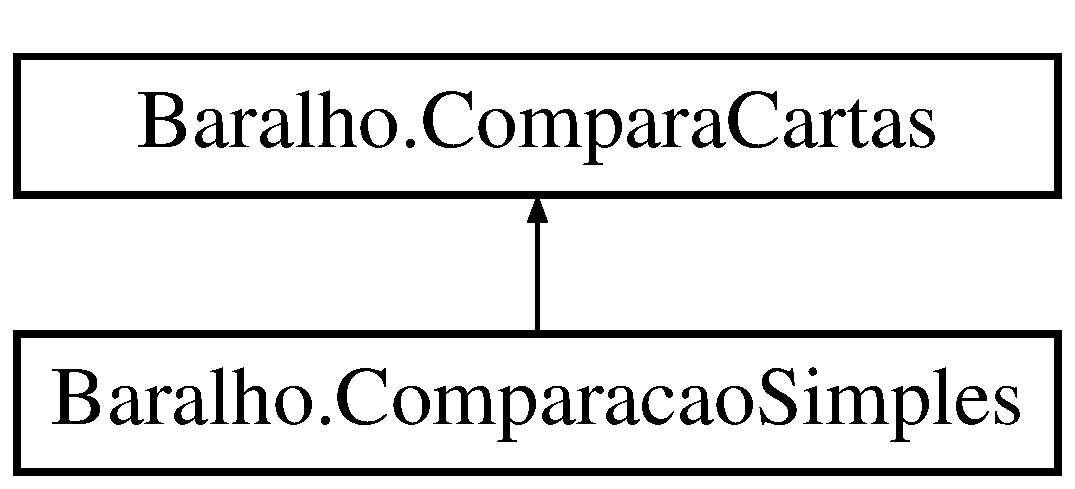
\includegraphics[height=2.000000cm]{class_baralho_1_1_comparacao_simples}
\end{center}
\end{figure}
\subsection*{\-Public \-Member \-Functions}
\begin{DoxyCompactItemize}
\item 
boolean \hyperlink{class_baralho_1_1_comparacao_simples_a1ea37c176e2c216536654b64ac8dc883}{e\-Maior} (\hyperlink{class_baralho_1_1_carta}{\-Carta} carta1, \hyperlink{class_baralho_1_1_carta}{\-Carta} carta2)
\end{DoxyCompactItemize}


\subsection{\-Detailed \-Description}
\-Comparação simples des cartas. \begin{DoxyAuthor}{\-Author}
\-Rafael 
\end{DoxyAuthor}


\subsection{\-Member \-Function \-Documentation}
\hypertarget{class_baralho_1_1_comparacao_simples_a1ea37c176e2c216536654b64ac8dc883}{
\index{\-Baralho\-::\-Comparacao\-Simples@{\-Baralho\-::\-Comparacao\-Simples}!e\-Maior@{e\-Maior}}
\index{e\-Maior@{e\-Maior}!Baralho::ComparacaoSimples@{\-Baralho\-::\-Comparacao\-Simples}}
\subsubsection[{e\-Maior}]{\setlength{\rightskip}{0pt plus 5cm}boolean \-Baralho.\-Comparacao\-Simples.\-e\-Maior (
\begin{DoxyParamCaption}
\item[{{\bf \-Carta}}]{carta1, }
\item[{{\bf \-Carta}}]{carta2}
\end{DoxyParamCaption}
)}}
\label{class_baralho_1_1_comparacao_simples_a1ea37c176e2c216536654b64ac8dc883}
\-Comparação simples para saber se uma carta tem peso maior que outra. 
\begin{DoxyParams}{\-Parameters}
{\em carta1} & -\/ \hyperlink{class_baralho_1_1_carta}{\-Carta} 1 para comparação. \\
\hline
{\em carta2} & -\/ \hyperlink{class_baralho_1_1_carta}{\-Carta} 2 para comparação. \\
\hline
\end{DoxyParams}
\begin{DoxyReturn}{\-Returns}
true -\/ se a carta 1 tiver peso maior que a carta 2. false -\/ se a carta 1 tiver peso menor ou igual que a carta 2. 
\end{DoxyReturn}


\-Implements \hyperlink{interface_baralho_1_1_compara_cartas_a805a502954c21d6fac410506bf81c955}{\-Baralho.\-Compara\-Cartas}.



\-The documentation for this class was generated from the following file\-:\begin{DoxyCompactItemize}
\item 
aula/111450026/\-Trabalho Baralho/\-Baralho/src/\-Baralho/\hyperlink{_comparacao_simples_8java}{\-Comparacao\-Simples.\-java}\end{DoxyCompactItemize}

\hypertarget{interface_baralho_1_1_compara_cartas}{
\section{Baralho.ComparaCartas Interface Reference}
\label{interface_baralho_1_1_compara_cartas}\index{Baralho::ComparaCartas@{Baralho::ComparaCartas}}
}
Inheritance diagram for Baralho.ComparaCartas:\begin{figure}[H]
\begin{center}
\leavevmode
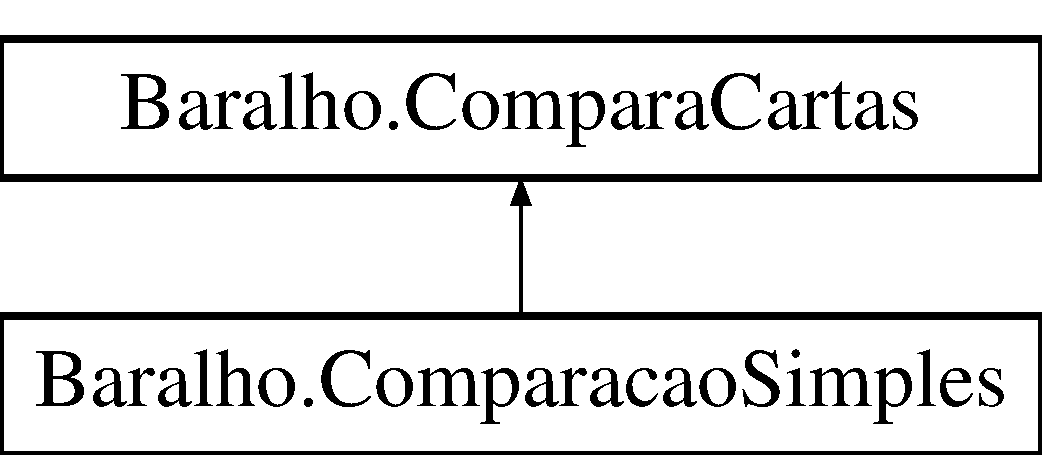
\includegraphics[height=2.000000cm]{interface_baralho_1_1_compara_cartas}
\end{center}
\end{figure}
\subsection*{Public Member Functions}
\begin{DoxyCompactItemize}
\item 
boolean \hyperlink{interface_baralho_1_1_compara_cartas_a805a502954c21d6fac410506bf81c955}{eMaior} (\hyperlink{class_baralho_1_1_carta}{Carta} carta1, \hyperlink{class_baralho_1_1_carta}{Carta} carta2)
\end{DoxyCompactItemize}


\subsection{Detailed Description}
Interface responsável pela comparação das cartas. \begin{DoxyAuthor}{Author}
Rafael 
\end{DoxyAuthor}


\subsection{Member Function Documentation}
\hypertarget{interface_baralho_1_1_compara_cartas_a805a502954c21d6fac410506bf81c955}{
\index{Baralho::ComparaCartas@{Baralho::ComparaCartas}!eMaior@{eMaior}}
\index{eMaior@{eMaior}!Baralho::ComparaCartas@{Baralho::ComparaCartas}}
\subsubsection[{eMaior}]{\setlength{\rightskip}{0pt plus 5cm}boolean Baralho.ComparaCartas.eMaior (
\begin{DoxyParamCaption}
\item[{{\bf Carta}}]{carta1, }
\item[{{\bf Carta}}]{carta2}
\end{DoxyParamCaption}
)}}
\label{interface_baralho_1_1_compara_cartas_a805a502954c21d6fac410506bf81c955}
Compara duas cartas pra saber se uma é maior do que a outra. 
\begin{DoxyParams}{Parameters}
{\em carta1} & -\/ \hyperlink{class_baralho_1_1_carta}{Carta} 1 da comparação. \\
\hline
{\em carta2} & -\/ \hyperlink{class_baralho_1_1_carta}{Carta} 2 da comparação. \\
\hline
\end{DoxyParams}
\begin{DoxyReturn}{Returns}
true -\/ se a carta 1 tiver peso maior. false -\/ se a carta 2 tiver peso menor. 
\end{DoxyReturn}


Implemented in \hyperlink{class_baralho_1_1_comparacao_simples_a1ea37c176e2c216536654b64ac8dc883}{Baralho.ComparacaoSimples}.



The documentation for this interface was generated from the following file:\begin{DoxyCompactItemize}
\item 
aula/111450026/Trabalho Baralho/Baralho/src/Baralho/\hyperlink{_compara_cartas_8java}{ComparaCartas.java}\end{DoxyCompactItemize}

\hypertarget{class_baralho_1_1_monte}{
\section{Baralho.Monte Class Reference}
\label{class_baralho_1_1_monte}\index{Baralho::Monte@{Baralho::Monte}}
}
Inheritance diagram for Baralho.Monte:\begin{figure}[H]
\begin{center}
\leavevmode
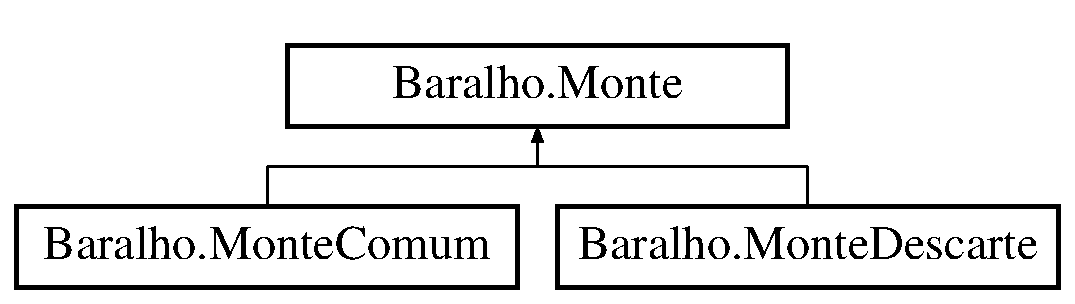
\includegraphics[height=2.000000cm]{class_baralho_1_1_monte}
\end{center}
\end{figure}
\subsection*{Public Member Functions}
\begin{DoxyCompactItemize}
\item 
void \hyperlink{class_baralho_1_1_monte_a9c0e60ff3e5adee7c73311dc639b726d}{initialize} (LinkedList$<$ \hyperlink{class_baralho_1_1_carta}{Carta} $>$ cartas)
\item 
boolean \hyperlink{class_baralho_1_1_monte_a62727fc8f2a5df78acf7ed256907d18d}{addCarta} (\hyperlink{class_baralho_1_1_carta}{Carta} carta)
\item 
void \hyperlink{class_baralho_1_1_monte_a54573fe9edbac3f8d9fca1fe1199debb}{addCarta} (\hyperlink{class_baralho_1_1_carta}{Carta} carta, int pos)  throws IndexOutOfBoundsException
\item 
void \hyperlink{class_baralho_1_1_monte_a64abc4bdca4718cb5e615154c562cf85}{removeCarta} (\hyperlink{class_baralho_1_1_carta}{Carta} carta)  throws CartaInexistenteException
\item 
void \hyperlink{class_baralho_1_1_monte_a81b0e1160db4914f5b1ba51fc068b1b9}{removeCarta} (int pos)  throws CartaInexistenteException 
\item 
LinkedList$<$ \hyperlink{class_baralho_1_1_carta}{Carta} $>$ \hyperlink{class_baralho_1_1_monte_a586ca35231a6c8a8634600df898f5ccc}{listaCartas} ()
\item 
\hyperlink{class_baralho_1_1_carta}{Carta} \hyperlink{class_baralho_1_1_monte_adeda515ad018d4975fbf054a37ab0f36}{obtemCarta} (int pos)  throws CartaInexistenteException
\item 
\hyperlink{class_baralho_1_1_carta}{Carta} \hyperlink{class_baralho_1_1_monte_ad724ab32986fbbc07e3d492aecfa2037}{obtemCarta} (\hyperlink{class_baralho_1_1_carta}{Carta} carta)  throws CartaInexistenteException 
\item 
void \hyperlink{class_baralho_1_1_monte_abd353fab5c3bfe77a070aafe7d905bec}{esvaziaMonte} ()
\item 
int \hyperlink{class_baralho_1_1_monte_a8768f18eb0e16b7a2be665360ad4afb5}{tamanho} ()
\end{DoxyCompactItemize}


\subsection{Detailed Description}
Classe abstrata que representa um monte do baralho. As posições das cartas do monte são consideradas de baixo para cima. \begin{DoxyAuthor}{Author}
Rafael 
\end{DoxyAuthor}


\subsection{Member Function Documentation}
\hypertarget{class_baralho_1_1_monte_a62727fc8f2a5df78acf7ed256907d18d}{
\index{Baralho::Monte@{Baralho::Monte}!addCarta@{addCarta}}
\index{addCarta@{addCarta}!Baralho::Monte@{Baralho::Monte}}
\subsubsection[{addCarta}]{\setlength{\rightskip}{0pt plus 5cm}boolean Baralho.Monte.addCarta (
\begin{DoxyParamCaption}
\item[{{\bf Carta}}]{carta}
\end{DoxyParamCaption}
)}}
\label{class_baralho_1_1_monte_a62727fc8f2a5df78acf7ed256907d18d}
Adiciona uma carta ao monte. 
\begin{DoxyParams}{Parameters}
{\em carta} & -\/ \hyperlink{class_baralho_1_1_carta}{Carta} a ser adicionda. \\
\hline
\end{DoxyParams}
\begin{DoxyReturn}{Returns}
true se a carta foi adicionada ou false caso contrário. 
\end{DoxyReturn}
\hypertarget{class_baralho_1_1_monte_a54573fe9edbac3f8d9fca1fe1199debb}{
\index{Baralho::Monte@{Baralho::Monte}!addCarta@{addCarta}}
\index{addCarta@{addCarta}!Baralho::Monte@{Baralho::Monte}}
\subsubsection[{addCarta}]{\setlength{\rightskip}{0pt plus 5cm}void Baralho.Monte.addCarta (
\begin{DoxyParamCaption}
\item[{{\bf Carta}}]{carta, }
\item[{int}]{pos}
\end{DoxyParamCaption}
)  throws IndexOutOfBoundsException}}
\label{class_baralho_1_1_monte_a54573fe9edbac3f8d9fca1fe1199debb}
Adiciona uma carta em uma posição específica do monte. 
\begin{DoxyParams}{Parameters}
{\em carta} & -\/ \hyperlink{class_baralho_1_1_carta}{Carta} a ser adicionada. \\
\hline
{\em pos} & -\/ Posição onde a carta será inserida. \\
\hline
\end{DoxyParams}

\begin{DoxyExceptions}{Exceptions}
{\em IndexOutOfBoundsException} & -\/ caso a posição em que a carta for inserida for fora dos limites do monte (menor que 0 ou maior que o tamanho do baralho). \\
\hline
\end{DoxyExceptions}
\hypertarget{class_baralho_1_1_monte_abd353fab5c3bfe77a070aafe7d905bec}{
\index{Baralho::Monte@{Baralho::Monte}!esvaziaMonte@{esvaziaMonte}}
\index{esvaziaMonte@{esvaziaMonte}!Baralho::Monte@{Baralho::Monte}}
\subsubsection[{esvaziaMonte}]{\setlength{\rightskip}{0pt plus 5cm}void Baralho.Monte.esvaziaMonte (
\begin{DoxyParamCaption}
{}
\end{DoxyParamCaption}
)}}
\label{class_baralho_1_1_monte_abd353fab5c3bfe77a070aafe7d905bec}
Retira todas as cartas do monte. \hypertarget{class_baralho_1_1_monte_a9c0e60ff3e5adee7c73311dc639b726d}{
\index{Baralho::Monte@{Baralho::Monte}!initialize@{initialize}}
\index{initialize@{initialize}!Baralho::Monte@{Baralho::Monte}}
\subsubsection[{initialize}]{\setlength{\rightskip}{0pt plus 5cm}void Baralho.Monte.initialize (
\begin{DoxyParamCaption}
\item[{LinkedList$<$ {\bf Carta} $>$}]{cartas}
\end{DoxyParamCaption}
)}}
\label{class_baralho_1_1_monte_a9c0e60ff3e5adee7c73311dc639b726d}
Inicializa o monte. As cartas que haviam nele são excluídas. 
\begin{DoxyParams}{Parameters}
{\em cartas} & -\/ Cartas do monte. \\
\hline
\end{DoxyParams}
\hypertarget{class_baralho_1_1_monte_a586ca35231a6c8a8634600df898f5ccc}{
\index{Baralho::Monte@{Baralho::Monte}!listaCartas@{listaCartas}}
\index{listaCartas@{listaCartas}!Baralho::Monte@{Baralho::Monte}}
\subsubsection[{listaCartas}]{\setlength{\rightskip}{0pt plus 5cm}LinkedList$<${\bf Carta}$>$ Baralho.Monte.listaCartas (
\begin{DoxyParamCaption}
{}
\end{DoxyParamCaption}
)}}
\label{class_baralho_1_1_monte_a586ca35231a6c8a8634600df898f5ccc}
Retorna as cartas do monte. \begin{DoxyReturn}{Returns}
-\/ cartas do monte. 
\end{DoxyReturn}
\hypertarget{class_baralho_1_1_monte_ad724ab32986fbbc07e3d492aecfa2037}{
\index{Baralho::Monte@{Baralho::Monte}!obtemCarta@{obtemCarta}}
\index{obtemCarta@{obtemCarta}!Baralho::Monte@{Baralho::Monte}}
\subsubsection[{obtemCarta}]{\setlength{\rightskip}{0pt plus 5cm}{\bf Carta} Baralho.Monte.obtemCarta (
\begin{DoxyParamCaption}
\item[{{\bf Carta}}]{carta}
\end{DoxyParamCaption}
)  throws {\bf CartaInexistenteException} }}
\label{class_baralho_1_1_monte_ad724ab32986fbbc07e3d492aecfa2037}
Retorna uma carta do monte. 
\begin{DoxyParams}{Parameters}
{\em carta} & -\/ A carta que se deseja obter do monte. \\
\hline
\end{DoxyParams}
\begin{DoxyReturn}{Returns}
A carta que se deseja, se ela constar no monte, ou null, caso contrário. 
\end{DoxyReturn}

\begin{DoxyExceptions}{Exceptions}
{\em CartaInexistenteException} & -\/ Caso a carta especificada não conste no monte. \\
\hline
\end{DoxyExceptions}
\hypertarget{class_baralho_1_1_monte_adeda515ad018d4975fbf054a37ab0f36}{
\index{Baralho::Monte@{Baralho::Monte}!obtemCarta@{obtemCarta}}
\index{obtemCarta@{obtemCarta}!Baralho::Monte@{Baralho::Monte}}
\subsubsection[{obtemCarta}]{\setlength{\rightskip}{0pt plus 5cm}{\bf Carta} Baralho.Monte.obtemCarta (
\begin{DoxyParamCaption}
\item[{int}]{pos}
\end{DoxyParamCaption}
)  throws {\bf CartaInexistenteException}}}
\label{class_baralho_1_1_monte_adeda515ad018d4975fbf054a37ab0f36}
Retorna a carta de uma posição do monte. 
\begin{DoxyParams}{Parameters}
{\em pos} & -\/ posição da carta no monte. \\
\hline
\end{DoxyParams}
\begin{DoxyReturn}{Returns}
A carta, se ela constar no monte, ou null, caso contrário. 
\end{DoxyReturn}

\begin{DoxyExceptions}{Exceptions}
{\em CartaInexistenteException} & -\/ Caso a posição especificada não aponte para uma carta do monte. \\
\hline
\end{DoxyExceptions}
\hypertarget{class_baralho_1_1_monte_a64abc4bdca4718cb5e615154c562cf85}{
\index{Baralho::Monte@{Baralho::Monte}!removeCarta@{removeCarta}}
\index{removeCarta@{removeCarta}!Baralho::Monte@{Baralho::Monte}}
\subsubsection[{removeCarta}]{\setlength{\rightskip}{0pt plus 5cm}void Baralho.Monte.removeCarta (
\begin{DoxyParamCaption}
\item[{{\bf Carta}}]{carta}
\end{DoxyParamCaption}
)  throws {\bf CartaInexistenteException}}}
\label{class_baralho_1_1_monte_a64abc4bdca4718cb5e615154c562cf85}
Remove uma carta do monte. 
\begin{DoxyParams}{Parameters}
{\em carta} & -\/ \hyperlink{class_baralho_1_1_carta}{Carta} a ser removida. \\
\hline
\end{DoxyParams}
\begin{DoxyReturn}{Returns}
true se a carta foi removida ou false caso contrário. 
\end{DoxyReturn}
\hypertarget{class_baralho_1_1_monte_a81b0e1160db4914f5b1ba51fc068b1b9}{
\index{Baralho::Monte@{Baralho::Monte}!removeCarta@{removeCarta}}
\index{removeCarta@{removeCarta}!Baralho::Monte@{Baralho::Monte}}
\subsubsection[{removeCarta}]{\setlength{\rightskip}{0pt plus 5cm}void Baralho.Monte.removeCarta (
\begin{DoxyParamCaption}
\item[{int}]{pos}
\end{DoxyParamCaption}
)  throws {\bf CartaInexistenteException} }}
\label{class_baralho_1_1_monte_a81b0e1160db4914f5b1ba51fc068b1b9}
Remove uma carta do monte. 
\begin{DoxyParams}{Parameters}
{\em pos} & -\/ posição da carta que irá ser removida. \\
\hline
\end{DoxyParams}
\begin{DoxyReturn}{Returns}
true se a carta foi removida ou false caso contrário. 
\end{DoxyReturn}
\hypertarget{class_baralho_1_1_monte_a8768f18eb0e16b7a2be665360ad4afb5}{
\index{Baralho::Monte@{Baralho::Monte}!tamanho@{tamanho}}
\index{tamanho@{tamanho}!Baralho::Monte@{Baralho::Monte}}
\subsubsection[{tamanho}]{\setlength{\rightskip}{0pt plus 5cm}int Baralho.Monte.tamanho (
\begin{DoxyParamCaption}
{}
\end{DoxyParamCaption}
)}}
\label{class_baralho_1_1_monte_a8768f18eb0e16b7a2be665360ad4afb5}
Retorna o tamanho do monte. \begin{DoxyReturn}{Returns}
tamanho do monte. 
\end{DoxyReturn}


The documentation for this class was generated from the following file:\begin{DoxyCompactItemize}
\item 
aula/111450026/Trabalho Baralho/Baralho/src/Baralho/\hyperlink{_monte_8java}{Monte.java}\end{DoxyCompactItemize}

\hypertarget{class_baralho_1_1_monte_comum}{
\section{Baralho.MonteComum Class Reference}
\label{class_baralho_1_1_monte_comum}\index{Baralho::MonteComum@{Baralho::MonteComum}}
}
Inheritance diagram for Baralho.MonteComum:\begin{figure}[H]
\begin{center}
\leavevmode
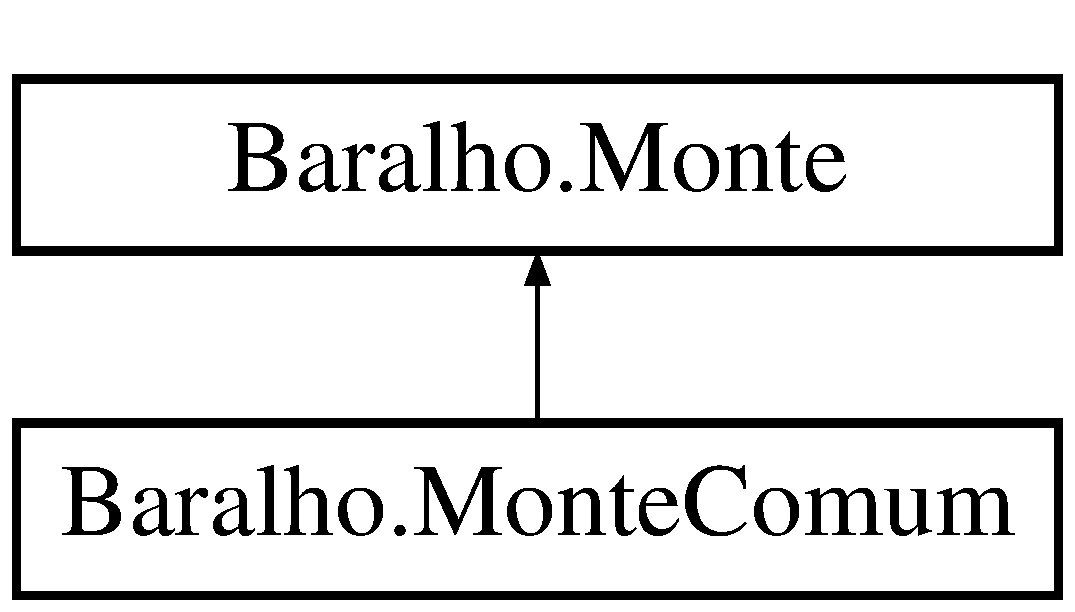
\includegraphics[height=2.000000cm]{class_baralho_1_1_monte_comum}
\end{center}
\end{figure}
\subsection*{Public Member Functions}
\begin{DoxyCompactItemize}
\item 
\hyperlink{class_baralho_1_1_monte_comum_af3664ab9b41ef3ea435033c9ae0132b9}{MonteComum} (LinkedList$<$ \hyperlink{class_baralho_1_1_carta}{Carta} $>$ cartas)
\item 
\hyperlink{class_baralho_1_1_monte_comum_ae5f9907b5ae8ec73544895110c7a0395}{MonteComum} ()
\end{DoxyCompactItemize}


\subsection{Detailed Description}
\hyperlink{class_baralho_1_1_monte}{Monte} comum de cartas. \begin{DoxyAuthor}{Author}
Rafael 
\end{DoxyAuthor}


\subsection{Constructor \& Destructor Documentation}
\hypertarget{class_baralho_1_1_monte_comum_af3664ab9b41ef3ea435033c9ae0132b9}{
\index{Baralho::MonteComum@{Baralho::MonteComum}!MonteComum@{MonteComum}}
\index{MonteComum@{MonteComum}!Baralho::MonteComum@{Baralho::MonteComum}}
\subsubsection[{MonteComum}]{\setlength{\rightskip}{0pt plus 5cm}Baralho.MonteComum.MonteComum (
\begin{DoxyParamCaption}
\item[{LinkedList$<$ {\bf Carta} $>$}]{cartas}
\end{DoxyParamCaption}
)}}
\label{class_baralho_1_1_monte_comum_af3664ab9b41ef3ea435033c9ae0132b9}
Método construtor. Chama initialize da classe monte. 
\begin{DoxyParams}{Parameters}
{\em cartas} & -\/ Cartas iniciais do monte. \\
\hline
\end{DoxyParams}
\hypertarget{class_baralho_1_1_monte_comum_ae5f9907b5ae8ec73544895110c7a0395}{
\index{Baralho::MonteComum@{Baralho::MonteComum}!MonteComum@{MonteComum}}
\index{MonteComum@{MonteComum}!Baralho::MonteComum@{Baralho::MonteComum}}
\subsubsection[{MonteComum}]{\setlength{\rightskip}{0pt plus 5cm}Baralho.MonteComum.MonteComum (
\begin{DoxyParamCaption}
{}
\end{DoxyParamCaption}
)}}
\label{class_baralho_1_1_monte_comum_ae5f9907b5ae8ec73544895110c7a0395}


The documentation for this class was generated from the following file:\begin{DoxyCompactItemize}
\item 
aula/111450026/Trabalho Baralho/Baralho/src/Baralho/\hyperlink{_monte_comum_8java}{MonteComum.java}\end{DoxyCompactItemize}

\hypertarget{class_baralho_1_1_monte_descarte}{
\section{\-Baralho.\-Monte\-Descarte \-Class \-Reference}
\label{class_baralho_1_1_monte_descarte}\index{\-Baralho.\-Monte\-Descarte@{\-Baralho.\-Monte\-Descarte}}
}
\-Inheritance diagram for \-Baralho.\-Monte\-Descarte\-:\begin{figure}[H]
\begin{center}
\leavevmode
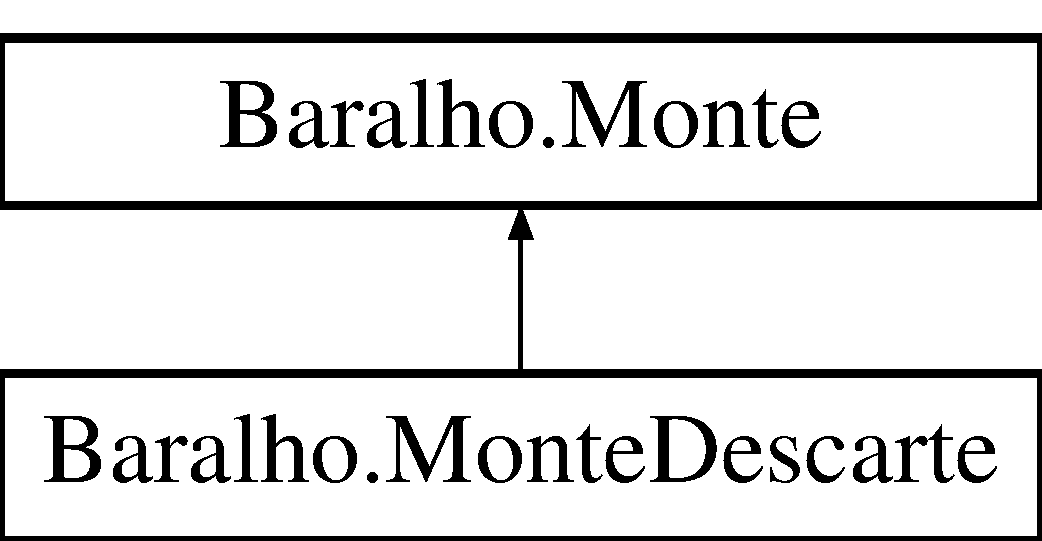
\includegraphics[height=2.000000cm]{class_baralho_1_1_monte_descarte}
\end{center}
\end{figure}
\subsection*{\-Public \-Member \-Functions}
\begin{DoxyCompactItemize}
\item 
\hyperlink{class_baralho_1_1_monte_descarte_a6dad15a6fd2ff4a535663173892936c7}{\-Monte\-Descarte} (\-Linked\-List$<$ \hyperlink{class_baralho_1_1_carta}{\-Carta} $>$ cartas)
\item 
\hyperlink{class_baralho_1_1_monte_descarte_aa36589f9e036fb890115e89e37b3b658}{\-Monte\-Descarte} ()
\item 
void \hyperlink{class_baralho_1_1_monte_descarte_a96b713dba347cd79bd944c0bef8a47ae}{exibir\-Carta} (\hyperlink{class_baralho_1_1_carta}{\-Carta} carta)
\item 
void \hyperlink{class_baralho_1_1_monte_descarte_a62c26b774387cec5611d723986c78ab0}{exibir\-Carta} (int pos)
\end{DoxyCompactItemize}


\subsection{\-Detailed \-Description}
\hyperlink{class_baralho_1_1_monte}{\-Monte} de descarte do baralho. \-Com ele é possível ver cartas sem que sejam retiradas do monte. \begin{DoxyAuthor}{\-Author}
pc 
\end{DoxyAuthor}


\subsection{\-Constructor \& \-Destructor \-Documentation}
\hypertarget{class_baralho_1_1_monte_descarte_a6dad15a6fd2ff4a535663173892936c7}{
\index{\-Baralho\-::\-Monte\-Descarte@{\-Baralho\-::\-Monte\-Descarte}!\-Monte\-Descarte@{\-Monte\-Descarte}}
\index{\-Monte\-Descarte@{\-Monte\-Descarte}!Baralho::MonteDescarte@{\-Baralho\-::\-Monte\-Descarte}}
\subsubsection[{\-Monte\-Descarte}]{\setlength{\rightskip}{0pt plus 5cm}\-Baralho.\-Monte\-Descarte.\-Monte\-Descarte (
\begin{DoxyParamCaption}
\item[{\-Linked\-List$<$ {\bf \-Carta} $>$}]{cartas}
\end{DoxyParamCaption}
)}}
\label{class_baralho_1_1_monte_descarte_a6dad15a6fd2ff4a535663173892936c7}
\-Método construtor. \-Chama initialize da classe monte. 
\begin{DoxyParams}{\-Parameters}
{\em cartas} & -\/ \-Cartas iniciais do monte. \\
\hline
\end{DoxyParams}
\hypertarget{class_baralho_1_1_monte_descarte_aa36589f9e036fb890115e89e37b3b658}{
\index{\-Baralho\-::\-Monte\-Descarte@{\-Baralho\-::\-Monte\-Descarte}!\-Monte\-Descarte@{\-Monte\-Descarte}}
\index{\-Monte\-Descarte@{\-Monte\-Descarte}!Baralho::MonteDescarte@{\-Baralho\-::\-Monte\-Descarte}}
\subsubsection[{\-Monte\-Descarte}]{\setlength{\rightskip}{0pt plus 5cm}\-Baralho.\-Monte\-Descarte.\-Monte\-Descarte (
\begin{DoxyParamCaption}
{}
\end{DoxyParamCaption}
)}}
\label{class_baralho_1_1_monte_descarte_aa36589f9e036fb890115e89e37b3b658}


\subsection{\-Member \-Function \-Documentation}
\hypertarget{class_baralho_1_1_monte_descarte_a96b713dba347cd79bd944c0bef8a47ae}{
\index{\-Baralho\-::\-Monte\-Descarte@{\-Baralho\-::\-Monte\-Descarte}!exibir\-Carta@{exibir\-Carta}}
\index{exibir\-Carta@{exibir\-Carta}!Baralho::MonteDescarte@{\-Baralho\-::\-Monte\-Descarte}}
\subsubsection[{exibir\-Carta}]{\setlength{\rightskip}{0pt plus 5cm}void \-Baralho.\-Monte\-Descarte.\-exibir\-Carta (
\begin{DoxyParamCaption}
\item[{{\bf \-Carta}}]{carta}
\end{DoxyParamCaption}
)}}
\label{class_baralho_1_1_monte_descarte_a96b713dba347cd79bd944c0bef8a47ae}
\-Exibe os dados da carta. 
\begin{DoxyParams}{\-Parameters}
{\em carta} & -\/ carta a ser exibida. \\
\hline
\end{DoxyParams}
\hypertarget{class_baralho_1_1_monte_descarte_a62c26b774387cec5611d723986c78ab0}{
\index{\-Baralho\-::\-Monte\-Descarte@{\-Baralho\-::\-Monte\-Descarte}!exibir\-Carta@{exibir\-Carta}}
\index{exibir\-Carta@{exibir\-Carta}!Baralho::MonteDescarte@{\-Baralho\-::\-Monte\-Descarte}}
\subsubsection[{exibir\-Carta}]{\setlength{\rightskip}{0pt plus 5cm}void \-Baralho.\-Monte\-Descarte.\-exibir\-Carta (
\begin{DoxyParamCaption}
\item[{int}]{pos}
\end{DoxyParamCaption}
)}}
\label{class_baralho_1_1_monte_descarte_a62c26b774387cec5611d723986c78ab0}
\-Exibe os dados da carta. 
\begin{DoxyParams}{\-Parameters}
{\em pos} & -\/ posição no monte da carta que se deseja exibir. \\
\hline
\end{DoxyParams}


\-The documentation for this class was generated from the following file\-:\begin{DoxyCompactItemize}
\item 
aula/111450026/\-Trabalho Baralho/\-Baralho/src/\-Baralho/\hyperlink{_monte_descarte_8java}{\-Monte\-Descarte.\-java}\end{DoxyCompactItemize}

\hypertarget{class_exce_xC3_xA7_xC3_xB5es_1_1_sequencia_invalida_exception}{
\section{\-Exceções.\-Sequencia\-Invalida\-Exception \-Class \-Reference}
\label{class_exce_xC3_xA7_xC3_xB5es_1_1_sequencia_invalida_exception}\index{\-Exceções.\-Sequencia\-Invalida\-Exception@{\-Exceções.\-Sequencia\-Invalida\-Exception}}
}
\subsection*{\-Public \-Member \-Functions}
\begin{DoxyCompactItemize}
\item 
\hyperlink{class_exce_xC3_xA7_xC3_xB5es_1_1_sequencia_invalida_exception_af6f229d3f7c1b2faaff12d7a0a71eba1}{\-Sequencia\-Invalida\-Exception} (\-String s)
\item 
\-String \hyperlink{class_exce_xC3_xA7_xC3_xB5es_1_1_sequencia_invalida_exception_a81cb14dec977306ce54527685ef130fc}{get\-Message} ()
\end{DoxyCompactItemize}


\subsection{\-Detailed \-Description}
\begin{DoxyAuthor}{\-Author}
rafael 
\end{DoxyAuthor}


\subsection{\-Constructor \& \-Destructor \-Documentation}
\hypertarget{class_exce_xC3_xA7_xC3_xB5es_1_1_sequencia_invalida_exception_af6f229d3f7c1b2faaff12d7a0a71eba1}{
\index{\-Exceções\-::\-Sequencia\-Invalida\-Exception@{\-Exceções\-::\-Sequencia\-Invalida\-Exception}!\-Sequencia\-Invalida\-Exception@{\-Sequencia\-Invalida\-Exception}}
\index{\-Sequencia\-Invalida\-Exception@{\-Sequencia\-Invalida\-Exception}!Exceções::SequenciaInvalidaException@{\-Exceções\-::\-Sequencia\-Invalida\-Exception}}
\subsubsection[{\-Sequencia\-Invalida\-Exception}]{\setlength{\rightskip}{0pt plus 5cm}\-Exceções.\-Sequencia\-Invalida\-Exception.\-Sequencia\-Invalida\-Exception (
\begin{DoxyParamCaption}
\item[{\-String}]{s}
\end{DoxyParamCaption}
)}}
\label{class_exce_xC3_xA7_xC3_xB5es_1_1_sequencia_invalida_exception_af6f229d3f7c1b2faaff12d7a0a71eba1}


\subsection{\-Member \-Function \-Documentation}
\hypertarget{class_exce_xC3_xA7_xC3_xB5es_1_1_sequencia_invalida_exception_a81cb14dec977306ce54527685ef130fc}{
\index{\-Exceções\-::\-Sequencia\-Invalida\-Exception@{\-Exceções\-::\-Sequencia\-Invalida\-Exception}!get\-Message@{get\-Message}}
\index{get\-Message@{get\-Message}!Exceções::SequenciaInvalidaException@{\-Exceções\-::\-Sequencia\-Invalida\-Exception}}
\subsubsection[{get\-Message}]{\setlength{\rightskip}{0pt plus 5cm}\-String \-Exceções.\-Sequencia\-Invalida\-Exception.\-get\-Message (
\begin{DoxyParamCaption}
{}
\end{DoxyParamCaption}
)}}
\label{class_exce_xC3_xA7_xC3_xB5es_1_1_sequencia_invalida_exception_a81cb14dec977306ce54527685ef130fc}


\-The documentation for this class was generated from the following file\-:\begin{DoxyCompactItemize}
\item 
aula/111450026/\-Trabalho Baralho/\-Baralho/src/\-Exceções/\hyperlink{_sequencia_invalida_exception_8java}{\-Sequencia\-Invalida\-Exception.\-java}\end{DoxyCompactItemize}

\chapter{File Documentation}
\hypertarget{_baralho_8java}{
\section{aula/111450026/\-Baralho/\-Baralho/\-Baralho.java \-File \-Reference}
\label{_baralho_8java}\index{aula/111450026/\-Baralho/\-Baralho/\-Baralho.\-java@{aula/111450026/\-Baralho/\-Baralho/\-Baralho.\-java}}
}
\subsection*{\-Classes}
\begin{DoxyCompactItemize}
\item 
class \hyperlink{class_baralho_1_1_baralho}{\-Baralho.\-Baralho}
\end{DoxyCompactItemize}
\subsection*{\-Packages}
\begin{DoxyCompactItemize}
\item 
package \hyperlink{namespace_baralho}{\-Baralho}
\end{DoxyCompactItemize}

\hypertarget{_carta_8java}{
\section{aula/111450026/\-Baralho/\-Baralho/\-Carta.java \-File \-Reference}
\label{_carta_8java}\index{aula/111450026/\-Baralho/\-Baralho/\-Carta.\-java@{aula/111450026/\-Baralho/\-Baralho/\-Carta.\-java}}
}
\subsection*{\-Classes}
\begin{DoxyCompactItemize}
\item 
class \hyperlink{class_baralho_1_1_carta}{\-Baralho.\-Carta}
\end{DoxyCompactItemize}
\subsection*{\-Packages}
\begin{DoxyCompactItemize}
\item 
package \hyperlink{namespace_baralho}{\-Baralho}
\end{DoxyCompactItemize}

\hypertarget{_comparacao_simples_8java}{
\section{aula/111450026/\-Baralho/\-Baralho/\-Comparacao\-Simples.java \-File \-Reference}
\label{_comparacao_simples_8java}\index{aula/111450026/\-Baralho/\-Baralho/\-Comparacao\-Simples.\-java@{aula/111450026/\-Baralho/\-Baralho/\-Comparacao\-Simples.\-java}}
}
\subsection*{\-Classes}
\begin{DoxyCompactItemize}
\item 
class \hyperlink{class_baralho_1_1_comparacao_simples}{\-Baralho.\-Comparacao\-Simples}
\end{DoxyCompactItemize}
\subsection*{\-Packages}
\begin{DoxyCompactItemize}
\item 
package \hyperlink{namespace_baralho}{\-Baralho}
\end{DoxyCompactItemize}

\hypertarget{_compara_cartas_8java}{
\section{aula/111450026/\-Baralho/\-Baralho/\-Compara\-Cartas.java \-File \-Reference}
\label{_compara_cartas_8java}\index{aula/111450026/\-Baralho/\-Baralho/\-Compara\-Cartas.\-java@{aula/111450026/\-Baralho/\-Baralho/\-Compara\-Cartas.\-java}}
}
\subsection*{\-Classes}
\begin{DoxyCompactItemize}
\item 
interface \hyperlink{interface_baralho_1_1_compara_cartas}{\-Baralho.\-Compara\-Cartas}
\end{DoxyCompactItemize}
\subsection*{\-Packages}
\begin{DoxyCompactItemize}
\item 
package \hyperlink{namespace_baralho}{\-Baralho}
\end{DoxyCompactItemize}

\hypertarget{_monte_8java}{
\section{aula/111450026/\-Baralho/\-Baralho/\-Monte.java \-File \-Reference}
\label{_monte_8java}\index{aula/111450026/\-Baralho/\-Baralho/\-Monte.\-java@{aula/111450026/\-Baralho/\-Baralho/\-Monte.\-java}}
}
\subsection*{\-Classes}
\begin{DoxyCompactItemize}
\item 
class \hyperlink{class_baralho_1_1_monte}{\-Baralho.\-Monte}
\end{DoxyCompactItemize}
\subsection*{\-Packages}
\begin{DoxyCompactItemize}
\item 
package \hyperlink{namespace_baralho}{\-Baralho}
\end{DoxyCompactItemize}

\hypertarget{_monte_comum_8java}{
\section{aula/111450026/\-Trabalho \-Baralho/\-Baralho/src/\-Baralho/\-Monte\-Comum.java \-File \-Reference}
\label{_monte_comum_8java}\index{aula/111450026/\-Trabalho Baralho/\-Baralho/src/\-Baralho/\-Monte\-Comum.\-java@{aula/111450026/\-Trabalho Baralho/\-Baralho/src/\-Baralho/\-Monte\-Comum.\-java}}
}
\subsection*{\-Classes}
\begin{DoxyCompactItemize}
\item 
class \hyperlink{class_baralho_1_1_monte_comum}{\-Baralho.\-Monte\-Comum}
\end{DoxyCompactItemize}
\subsection*{\-Packages}
\begin{DoxyCompactItemize}
\item 
package \hyperlink{namespace_baralho}{\-Baralho}
\end{DoxyCompactItemize}

\hypertarget{_monte_descarte_8java}{
\section{aula/111450026/\-Trabalho \-Baralho/\-Baralho/src/\-Baralho/\-Monte\-Descarte.java \-File \-Reference}
\label{_monte_descarte_8java}\index{aula/111450026/\-Trabalho Baralho/\-Baralho/src/\-Baralho/\-Monte\-Descarte.\-java@{aula/111450026/\-Trabalho Baralho/\-Baralho/src/\-Baralho/\-Monte\-Descarte.\-java}}
}
\subsection*{\-Classes}
\begin{DoxyCompactItemize}
\item 
class \hyperlink{class_baralho_1_1_monte_descarte}{\-Baralho.\-Monte\-Descarte}
\end{DoxyCompactItemize}
\subsection*{\-Packages}
\begin{DoxyCompactItemize}
\item 
package \hyperlink{namespace_baralho}{\-Baralho}
\end{DoxyCompactItemize}

\hypertarget{_naipe_8java}{
\section{aula/111450026/Trabalho Baralho/Baralho/src/Baralho/Naipe.java File Reference}
\label{_naipe_8java}\index{aula/111450026/Trabalho Baralho/Baralho/src/Baralho/Naipe.java@{aula/111450026/Trabalho Baralho/Baralho/src/Baralho/Naipe.java}}
}
\subsection*{Packages}
\begin{DoxyCompactItemize}
\item 
package \hyperlink{namespace_baralho}{Baralho}
\end{DoxyCompactItemize}
\subsection*{Enumerations}
\begin{DoxyCompactItemize}
\item 
enum \hyperlink{namespace_baralho_ab887857dcb81ef6672322ce80039b905}{Baralho.Naipe} \{ \hyperlink{namespace_baralho_ab887857dcb81ef6672322ce80039b905}{Baralho.OUROS}, 
\hyperlink{namespace_baralho_ab887857dcb81ef6672322ce80039b905}{Baralho.peso}, 
\hyperlink{namespace_baralho_ab887857dcb81ef6672322ce80039b905}{Baralho.peso}, 
\hyperlink{namespace_baralho_ab887857dcb81ef6672322ce80039b905}{Baralho.peso}
 \}
\end{DoxyCompactItemize}

\hypertarget{_carta_inexistente_exception_8java}{
\section{aula/111450026/\-Trabalho \-Baralho/\-Baralho/src/\-Exceções/\-Carta\-Inexistente\-Exception.java \-File \-Reference}
\label{_carta_inexistente_exception_8java}\index{aula/111450026/\-Trabalho Baralho/\-Baralho/src/\-Exceções/\-Carta\-Inexistente\-Exception.\-java@{aula/111450026/\-Trabalho Baralho/\-Baralho/src/\-Exceções/\-Carta\-Inexistente\-Exception.\-java}}
}
\subsection*{\-Classes}
\begin{DoxyCompactItemize}
\item 
class \hyperlink{class_exce_xC3_xA7_xC3_xB5es_1_1_carta_inexistente_exception}{\-Exceções.\-Carta\-Inexistente\-Exception}
\end{DoxyCompactItemize}
\subsection*{\-Packages}
\begin{DoxyCompactItemize}
\item 
package \hyperlink{namespace_exce_xC3_xA7_xC3_xB5es}{\-Exceções}
\end{DoxyCompactItemize}

\hypertarget{_carta_invalida_exception_8java}{
\section{aula/111450026/\-Baralho/\-Exceções/\-Carta\-Invalida\-Exception.java \-File \-Reference}
\label{_carta_invalida_exception_8java}\index{aula/111450026/\-Baralho/\-Exceções/\-Carta\-Invalida\-Exception.\-java@{aula/111450026/\-Baralho/\-Exceções/\-Carta\-Invalida\-Exception.\-java}}
}
\subsection*{\-Classes}
\begin{DoxyCompactItemize}
\item 
class \hyperlink{class_exce_xC3_xA7_xC3_xB5es_1_1_carta_invalida_exception}{\-Exceções.\-Carta\-Invalida\-Exception}
\end{DoxyCompactItemize}
\subsection*{\-Packages}
\begin{DoxyCompactItemize}
\item 
package \hyperlink{namespace_exce_xC3_xA7_xC3_xB5es}{\-Exceções}
\end{DoxyCompactItemize}

\hypertarget{_sequencia_invalida_exception_8java}{
\section{aula/111450026/\-Trabalho \-Baralho/\-Baralho/src/\-Exceções/\-Sequencia\-Invalida\-Exception.java \-File \-Reference}
\label{_sequencia_invalida_exception_8java}\index{aula/111450026/\-Trabalho Baralho/\-Baralho/src/\-Exceções/\-Sequencia\-Invalida\-Exception.\-java@{aula/111450026/\-Trabalho Baralho/\-Baralho/src/\-Exceções/\-Sequencia\-Invalida\-Exception.\-java}}
}
\subsection*{\-Classes}
\begin{DoxyCompactItemize}
\item 
class \hyperlink{class_exce_xC3_xA7_xC3_xB5es_1_1_sequencia_invalida_exception}{\-Exceções.\-Sequencia\-Invalida\-Exception}
\end{DoxyCompactItemize}
\subsection*{\-Packages}
\begin{DoxyCompactItemize}
\item 
package \hyperlink{namespace_exce_xC3_xA7_xC3_xB5es}{\-Exceções}
\end{DoxyCompactItemize}

\printindex
\end{document}
